% ─── Slide: INT4 PTQ journey ──────────────────────────────────────────────────
\begin{frame}{INT4 Pure PTQ: A Stepwise Story}
  \begin{columns}[T]
    \begin{column}{0.48\textwidth}
      \textbf{Each step fixes one failure mode:}

      \begin{enumerate}
        \small
        \item \textbf{Baseline INT4 (128 samples):}
          $\adcppl = 2355$ — catastrophic; INT4 overfits on 128 samples.

        \item \textbf{Propagation (128 samples):}
          $\adcppl = 204$ — better, but bypass \emph{degrades} (transforms
          over-specialise for corrupted inputs).

        \item \textbf{Propagation (512+ samples):}
          $\adcppl = 40.6$ — samples are the dominant lever.

        \item \textbf{Partial propagation $\alpha = 0.5$ (1024 samples):}
          $\adcppl = 31.2$ — mixed FP+quant loss is better than either alone.

        \item \textbf{Bounded LET diag + $\alpha = 0.5$:}
          $\adcppl = 27.56$ — diagonal scaling adds expressivity.

        \item \textbf{Staged training (MLP diag $\to$ attn diag):}
          $\adcppl = 27.60$, $\bypass = 18.50$ — cleanest bypass yet.
      \end{enumerate}

      \vspace{0.5em}
      \begin{alertblock}{Key insight}
        Bin-centre loss is \worse{harmful} for INT4
        ($\delta_{\mathrm{INT4}} \approx 515$: penalty dominates \& destabilises).
      \end{alertblock}
    \end{column}
    \begin{column}{0.48\textwidth}
      % plot_int4_ptq_progression.pdf
      \iffalse
        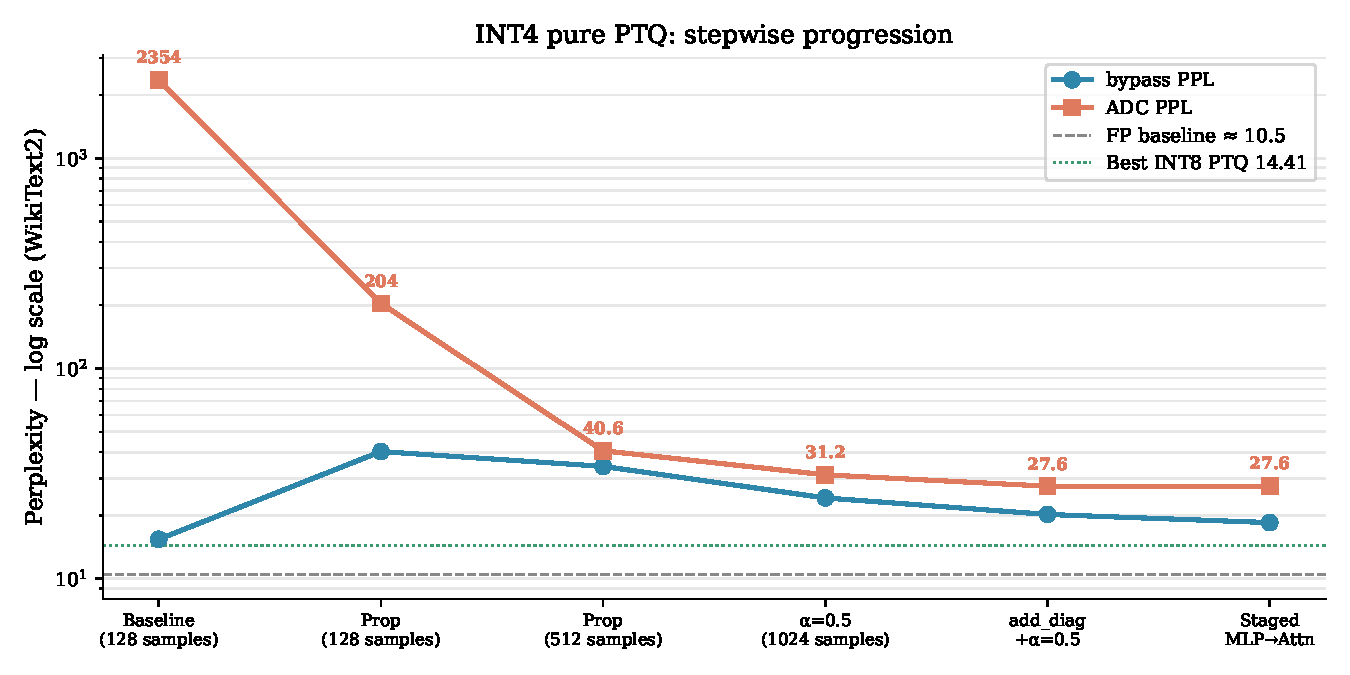
\includegraphics[width=\linewidth]{figs/plot_int4_ptq_progression.pdf}
      \else
        \figplaceholder[0.70\textheight]{Step plot (x = method index 1--6,
          log y-axis = PPL).
          Two lines: bypass PPL (blue) and ADC PPL (orange).
          Annotate each step with the key change.
          Show FP baseline as dashed line at 10.5 and INT8-prop+center at 14.41.
          Key numbers: 2355, 204, 40.6, 31.2, 27.56, 27.60.}
      \fi
    \end{column}
  \end{columns}
\end{frame}
